\documentclass[conference]{IEEEtran}

\usepackage[T1]{fontenc}
\usepackage{amsmath}
\usepackage{amsfonts}
\usepackage{graphicx}

\title{Scalar SMU for Native Online Attention}

\author{\IEEEauthorblockN{xt}}

\begin{document}

\maketitle

\begin{abstract}
Abstract placeholder.
\end{abstract}

\section{Introduction}
% TODO: Add the introduction.

\section{Native Online Attention and Design Motivation}

\subsection{Native Online Attention}
Attention computes a weighted aggregation of value vectors according to the
similarity between a query and a set of keys. A conventional implementation
materializes the attention scores and normalized probability matrix before
performing the final weighted value accumulation. Online attention instead
processes the score matrix in tiles and incrementally maintains the
normalization state and partial output. This organization avoids materializing
the complete attention probability matrix and is particularly suitable for
memory-constrained execution.

For a query row, let a previously accumulated attention state be represented
by the triplet
\[
(m,l,\mathbf{O}),
\]
where $m$ is the running maximum of the processed scores, $l$ is the
corresponding exponential normalization term, and
$\mathbf{O}\in\mathbb{R}^{D}$ is the normalized output vector. For a newly
processed score tile, the tile-local state is similarly denoted as
\[
(m_t,l_t,\mathbf{O}_t).
\]

The previous and tile-local states are merged without reconstructing the
probabilities of earlier tiles. The new maximum is first computed as
\[
m'=\max(m,m_t).
\]
The two normalization contributions are then rescaled to the common maximum,
\[
\tilde{l}_{\mathrm{old}}=l\exp(m-m'),
\]
\[
\tilde{l}_{\mathrm{tile}}=l_t\exp(m_t-m'),
\]
and the updated normalization state becomes
\[
l'=\tilde{l}_{\mathrm{old}}+\tilde{l}_{\mathrm{tile}}.
\]
This recurrence also produces the two normalized rescaling weights
\[
w_{\mathrm{old}}=\frac{\tilde{l}_{\mathrm{old}}}{l'},\qquad
w_{\mathrm{tile}}=\frac{\tilde{l}_{\mathrm{tile}}}{l'}.
\]
The output state can therefore be updated as
\[
\mathbf{O}'=w_{\mathrm{old}}\mathbf{O}
  +w_{\mathrm{tile}}\mathbf{O}_t.
\]

The first tile does not require a merge operation and directly initializes the
running state. Each subsequent tile executes one recurrence to obtain the
updated scalar state and the two rescaling weights, followed by an update over
the $D$-dimensional output vector. Since the output is maintained in normalized
form after every merge, no additional final normalization pass is required.

Although these operations jointly implement one logical online merge, they
exhibit substantially different computational structures. This distinction
forms the basis of the HW/SW partition developed in this work.

\subsection{Execution Characteristics}
Fig.~\ref{fig:motivation} illustrates the decomposition of a native
online-attention merge into two components: a state-dependent scalar
recurrence and a regular vector output update. The former updates $m$ and $l$
and generates $w_{\mathrm{old}}$ and $w_{\mathrm{tile}}$, whereas the latter
applies these weights independently to the $D$ output elements.

\begin{figure*}[t]
\centering
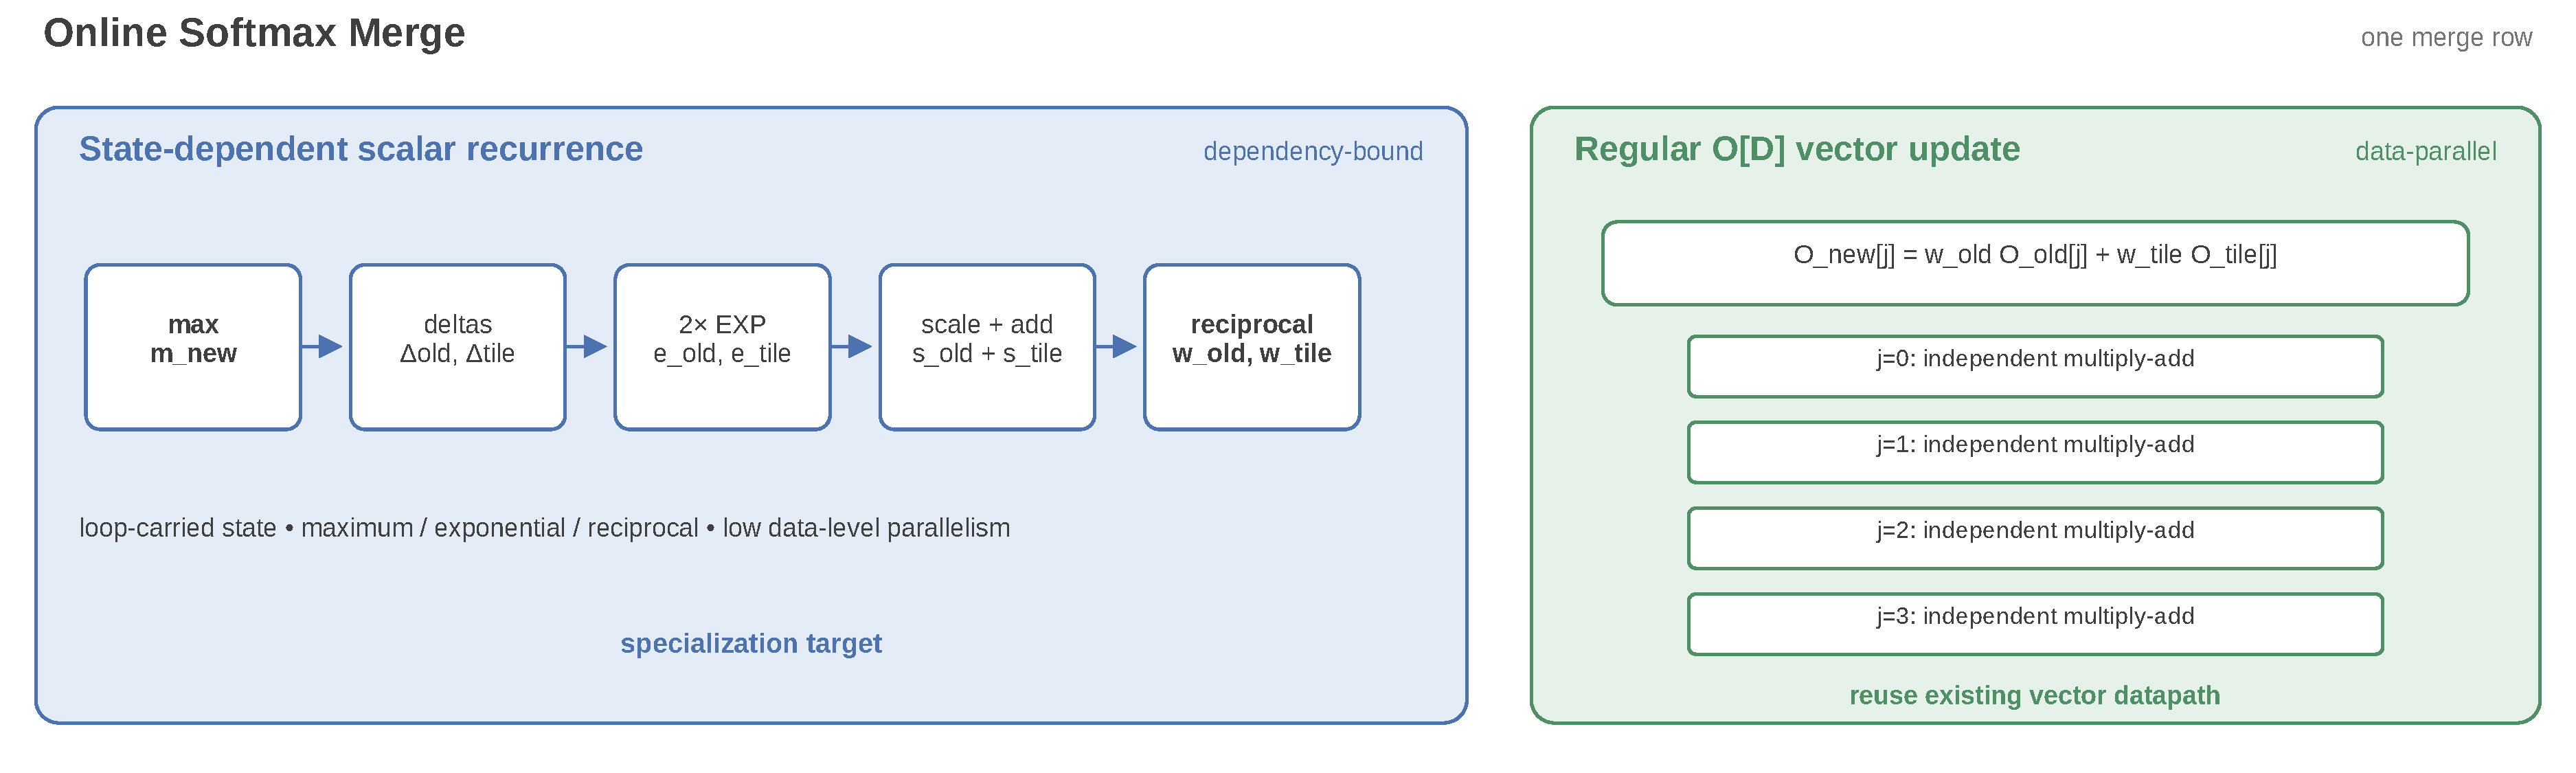
\includegraphics[width=\textwidth]{../experiments/plots/figure1_computation_decomposition.pdf}
\caption{Execution decomposition of a native online-attention merge. The
state-dependent recurrence updates $m$ and $l$ and generates two scalar
rescaling weights, while the regular $D$-dimensional output update remains
mapped to the existing RVV datapath.}
\label{fig:motivation}
\end{figure*}

The recurrence contains several properties that limit the regular data-level
parallelism available within a single merge. First, the new state depends on
the state produced by previous tiles, forming a loop-carried dependency across
successive merge operations. Second, its computation includes maximum
selection, exponential rescaling, accumulation, and normalization. These
operations form a short heterogeneous dependency chain rather than a uniform
element-wise loop. Third, the amount of scalar work associated with the
recurrence does not scale with the output dimension $D$. Increasing $D$
therefore does not expose additional parallel recurrence elements that could
naturally occupy the vector lanes.

The output update has the opposite structure. For each element $j$,
\[
O'[j]=w_{\mathrm{old}}O[j]+w_{\mathrm{tile}}O_t[j],\qquad 0\leq j<D,
\]
and all $D$ elements use the same pair of scalar weights. Once the recurrence
has completed, the update contains no inter-element dependency and consists
primarily of regular floating-point multiply-add operations. It therefore
exposes explicit $D$-dimensional data parallelism and naturally maps to the
existing RVV execution resources.

This decomposition suggests that treating the entire merge as a single
acceleration target would unnecessarily duplicate functionality already
provided by the vector processor. Conversely, retaining the complete operation
in software leaves the state-dependent nonlinear recurrence on the scalar
execution path. We instead consider the recurrence and the output update as
two distinct execution domains: the former is a compact, dependency-dominated
operation suitable for specialized execution, while the latter is a regular
vector computation that can continue to use the existing RVV datapath.

This distinction is important to the scope of the proposed accelerator. The
objective is not to replace the vector processor or to offload the complete
attention computation. Score generation, tile-local state construction, and
the $D$-dimensional output update remain part of the programmable execution
path. The specialization targets only the state-dependent merge recurrence
that connects consecutive online-attention tiles.

\subsection{Design Objectives}
The execution characteristics above lead to three design objectives.

First, the accelerator should follow a \textbf{selective specialization}
strategy. Only the state-dependent recurrence should be moved to dedicated
hardware, while the regular output update should reuse the existing vector
processor. Such a partition preserves the programmability and established
data-parallel execution capability of RVV while avoiding the need to
reproduce a $D$-wide vector datapath inside the accelerator.

Second, the specialized recurrence unit should remain sufficiently lightweight
for cluster-local integration. The recurrence combines maximum computation,
exponentiation, accumulation, and normalization, but these stages do not
necessarily require a uniform numerical representation. The accelerator should
therefore exploit stage-specific numerical requirements to reduce hardware cost
while maintaining the accuracy required by the online-attention state. This
motivates the stage-aware mixed-precision design presented in Section~III.

Third, the HW/SW interface should reflect the temporal structure of online
attention. Some accelerator parameters remain unchanged across all merges of a
workload, whereas a merge invocation itself occurs repeatedly as new tiles are
processed. Reprogramming workload-persistent state through a conventional
control path for every merge would introduce redundant software orchestration.
The interface should therefore separate persistent context establishment from
per-merge execution and should minimize software management of the dynamically
alternating recurrence state.

Based on these objectives, we adopt a fine-grained HW/SW partition in which a
cluster-local mixed-precision scalar SMU executes the state-dependent
recurrence, while the existing Spatz/RVV datapath performs the
$D$-dimensional output update. The accelerator is exposed through a
lightweight RISC-V interface that separates workload-persistent configuration
from individual merge invocations and maintains the alternating scalar
recurrence state in hardware. Section~III describes this architecture and
programming model in detail.

\section{Architecture and HW/SW Co-Design}

\subsection{System Overview and HW/SW Partition}
% TODO: Present the system overview and HW/SW partition.

\subsection{Stage-Aware Mixed-Precision SMU}
% TODO: Describe the stage-aware mixed-precision SMU.

\subsection{OMERGE Per-Merge Invocation}
% TODO: Describe the OMERGE invocation interface.

\subsection{OMCFG Persistent Configuration}
% TODO: Describe persistent configuration through OMCFG.

\subsection{Hardware-Maintained Dynamic State}
% TODO: Describe the hardware-maintained dynamic state.

\section{Evaluation}

\subsection{Experimental Setup and Measurement Scope}
% TODO: Define the experimental setup and measurement scope.

\subsection{Numerical Fidelity and Standalone SMU Cost}
% TODO: Report numerical fidelity and standalone SMU cost.

\subsection{Native Online Attention Performance}
% TODO: Report native online attention performance.

\subsection{HW/SW Partition Ablation}
% TODO: Report the HW/SW partition ablation.

\subsection{ISA Interface Evaluation}
% TODO: Evaluate the ISA interface.

\subsection{Explicit-P Negative Control}
% TODO: Report the explicit-P negative control.

\section{Related Work}

\subsection{Softmax and Nonlinear Acceleration}
% TODO: Discuss softmax and nonlinear acceleration.

\subsection{RISC-V Domain-Specific Acceleration}
% TODO: Discuss RISC-V domain-specific acceleration.

\subsection{HW/SW Co-Design for AI Acceleration}
% TODO: Discuss HW/SW co-design for AI acceleration.

\section{Conclusion}
% TODO: Add the conclusion.

\begin{thebibliography}{00}

\bibitem{placeholder}
Reference placeholder.

\end{thebibliography}

\end{document}
